\begin{minipage}[t]{.6\linewidth}
  The \textbf{synthesis objective} is to \textbf{shape the norm of two filters}
  while ensuring their \textbf{complementary property}.
  This is equivalent to the conditions on the right where \(H_1(s)\) and
  \(H_2(s)\) are stable transfer function.

  \bigskip

  $W_1(s)$ and $W_2(s)$ are \textbf{weighting functions} that are used to define
  wanted \textbf{upper bound of the complementary filter norms}.
  They should be \textbf{proper}, \textbf{stable} and \textbf{minimum phase}
  transfer functions.
\end{minipage}\hfill%
\begin{minipage}[t]{.38\linewidth}
  \vspace{-1em}
  \[ \tcmbox{\begin{align*}
       &H_1(s) + H_2(s) = 1 \\
       &|H_1(j\omega)| \le \frac{1}{|W_1(j\omega)|} \quad \forall\omega \\
       &|H_2(j\omega)| \le \frac{1}{|W_2(j\omega)|} \quad \forall\omega
     \end{align*}} \]
\end{minipage}

\bigskip

\begin{minipage}[t]{0.47\linewidth}
  This optimization problem is written as a \textbf{standard} \(\mathcal{H}_\infty\)
  \textbf{problem} (Fig.~\ref{fig:h_infinity_robust_fusion}).

  The \(\mathcal{H}_\infty\) synthesis applied to \(P(s)\) generates
  a stable filter \(H_2(s)\) such that the \(\mathcal{H}_\infty\) norm from \(w\) to \([z_1, \ z_2]\)
  is less than one.
  By defining \(H_1(s) \triangleq 1 - H_2(s)\), this is equivalent to the
  synthesis objective described above.
  \begin{tikzfigure}[$\mathcal{H}_\infty$ synthesis of
    complementary filters]
    \label{fig:h_infinity_robust_fusion}
    \centering
    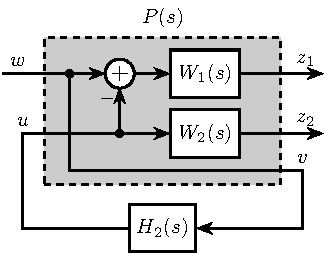
\includegraphics[scale=1.8]{figs/h_infinity_robust_fusion.pdf}
  \end{tikzfigure}
\end{minipage}\hfill
\begin{minipage}[t]{0.49\linewidth}
  This \(\mathcal{H}_\infty\) synthesis is first applied for the design of simple complementary
  filters (Fig.~\ref{fig:hinf_synthesis_results}).

  \begin{tikzfigure}[Frequency response of the weighting functions and
    complementary filters obtained using $\mathcal{H}_\infty$ synthesis]
    \label{fig:hinf_synthesis_results}
    \centering
    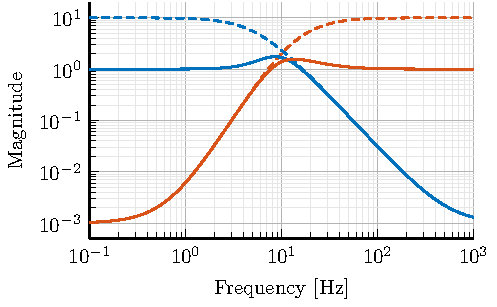
\includegraphics[width=\linewidth]{figs/hinf_synthesis_results.pdf}
  \end{tikzfigure}
\end{minipage}

%%% Local Variables:
%%% TeX-master: "poster"
%%% End: